\documentclass{article}
\usepackage{styles}

\title{Image Processing\\
    Lab 2}
\author{Kevin Gevers (s25595987) \\ Jeroen Overschie (s2995697)}
\date{\today}

\begin{document}

\maketitle

Note, that all used source code can be found attached next to this report's pdf file. Its structure should be self-explanatory; all requested functions are named accordingly and any extra functions are explained in the report. Note that (almost) every function has a corresponding test script, which is named just like its function, but with a suffix '\texttt{\_test}'. Where possible, we followed the terminology from the book \citep{gonzalez2008digital} for variable naming.

\section*{Exercise 1}
\subsection*{(a)}
For the first exercise of this lab we had to compute the \textit{centered Fourier spectrum} of the input image \textit{characters.tif}. This involves three steps, first we need to apply the fourier transformation, then we need to center it, and lastly we need to take the magnitude of it. 

The first step is to calculate the 2D Discrete Fourier Transform (DFT) of the image, according to Formula \ref{eq:fourier2d} (Eq.4-67 in the book). Since we are allowed to use Matlab's \texttt{fft2} function we did not implement this ourselves.

\begin{equation}\label{eq:fourier2d}
    F(u, v)=\sum_{x=0}^{M-1} \sum_{y=0}^{N-1} f(x, y) e^{-j 2 \pi(u x / M+v y / N)}
\end{equation}

For the second step we need to center the Fourier transform. For displaying and filtering purposes we want to move the four quarter periods (shown with the dotted lines on the left side of Figure \ref{fig:fouriershiftFromBook}), so that we have one full period instead. To do this we need to apply Formula \ref{eq:fouriershift} (Eq.4-76 in the book). Seeing as we are allowed to use Matlab's \textit{fftshift} function we did not have to implement this ourselves.

\begin{figure}[h]
    \centering
    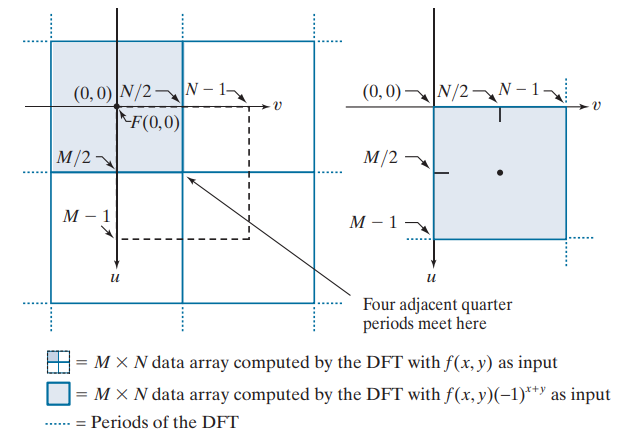
\includegraphics[width=0.7\textwidth]{Assignment_2/output_plots/centered_fourier_spectrum_book.png}
    \caption{Image showing what is happening to the image when the Fourier transform is being centered \cite{gonzalez2008digital}.}
    \label{fig:fouriershiftFromBook}
\end{figure}

\begin{equation}\label{eq:fouriershift}
    f(x, y)(-1)^{x+y} \Leftrightarrow F(u-M / 2, v-N / 2)
\end{equation}

The third and final step is taking the magnitude of the centered Fourier transform, which gives us the spectrum. The magnitude of each pixel is the absolute value of each pixel. Since the centered Fourier transform consists of complex numbers we need to apply Formula \ref{eq:absComplex} (Eq.4-87 in the book). This gives us the polar representation of the pixel and can be used to visualize the spectrum. Matlab's standard function \texttt{abs} handles complex numbers using this formula, so we again did not implement this.

\begin{equation}\label{eq:absComplex}
    |F(u, v)|=\sqrt{R^{2}(u, v)+I^{2}(u, v)}
\end{equation}

\newpage
\subsection*{(b)}
Now that we have the centered Fourier spectrum of the input image we can visualize it. The centered Fourier spectrum is visualized in Figure \ref{fig:exercise1}b, but is near impossible to see (please use the matlab code to get an interactive image if you do want to see it properly). To make sure the spectrum is easily visible we use a log transformation. In Figure \ref{fig:exercise1}d the log transformation of the spectrum can be seen and is much easier to interpret. Figure \ref{fig:exercise1}a and \ref{fig:exercise1}c show the non-centered Fourier spectrum without and with the log transformation respectively.

\begin{figure}[h]
    \centering
    \includesvg[width=\textwidth]{Assignment_2/output_plots/exercise1.svg}
    \caption{(a) non-centered Fourier spectrum. (b) centered Fourier spectrum. (c) log transformation of the non-centered Fourier spectrum. (d) log transformation of the centered Fourier spectrum.}
    \label{fig:exercise1}
\end{figure}

\subsection*{(c)}
The last part of the exercise simply wants us to use the result from (a) to compute the average value of the image. Formula \ref{eq:zeroFreqProp} (Eq.4-92 in the book) shows that the zero-frequency term of the DFT is proportional to the mean of the original image. The following steps are clearly outlined in \ding{118} Listing \ref{code:exercise1}. The average of the original image is $0.7997$ and using Formula \ref{eq:zeroFreqProp} we determined that $M N \bar{f} = 3.7855e+05$. By selecting the middle pixel of the centered Fourier spectrum (the result of (a)) we get the zero-frequency term of our result, which is also $3.7855e+05$. We divide that by the dimensions of the image ($M$ and $N$) and get the average value of the original image again: $0.7997$.

\begin{equation}\label{eq:zeroFreqProp}
    \begin{aligned}
    F(0,0) &=M N \frac{1}{M N} \sum_{x=0}^{M-1} \sum_{y=0}^{N-1} f(x, y) \\
    &=M N \bar{f}
    \end{aligned}
\end{equation}

The resulting code for the entire exercise can be seen in \ding{118} Listing \ref{code:exercise1}.

\newpage
\section*{Exercise 2}
\subsection*{(a)} In this exercise we are asked to implement a \textit{Butterworth Highpass Filter} (BHPF) transfer function. To do this, we first built a distance function $D$ as according to Eq (4-112):

\[
D(u,v)=[(u-P/2)^2+(v-Q/2)^2]^{1/2}
\]

This function computes the distance for some given coordinate $(u, v)$ to the centre of the $P \times Q$ frequency rectangle (note the sizes of $P$ and $Q$ in Eqs. (4-100) and (4-101): $2M$ and $2N$, respectively), which can be intuitively understood as the Euclidean distance in two-dimensional u/v space. The distance function is implemented in \ding{118} Listing~\ref{code:IPfreqrectdists}. Once we have our distance function, we can define our Butterworth highpass filter transfer function, Eq (4-121):

\[
H(u, v) = \frac{1}{1+[D_0 / D(u, v)]^{1/2}}
\]

Where $D_0$ is the cutoff frequency and the order is given by $n$. For the implementation of this transfer function, see \ding{118} Listing~\ref{code:IPbhpf}. We are now able to create and visualize the filter we just built. If we take some appropriately-sized matrix, e.g. of 500x500 size, we can visualize what the transfer function looks like. We iterate the function over (1) a 3D $u$/$v$ space with the z-coordinate set as the function value $H(u, v)$, (2) a 2D $u$/$v$ with the function value $H(u, v)$ set as the grayscale color intensity and finally (3) a cross-section of the transfer function, made over the constant value $v = 500$ and letting $u$ range from 500 to 1000, i.e. $u = [500, 501, ..., 1000]$. We set the x axis as the distance function value, $D(u, v)$, indicating how far off the given point is from the center. See Figure~\ref{fig:bhpf}.

\begin{figure}[ht]
    \centering
    \includesvg[width=\textwidth]{Assignment_2/output_plots/bhpf_500x500.svg}
    \caption{Visualization of the BHPF transfer function $H(u, v)$. (1) H in 3D space, (2) H as a grayscale intensity value in a 2D space and (3) a cross-section of H versus the distance function D.}
    \label{fig:bhpf}
\end{figure}

Due to a high amount of curiosity, we were wondering whether we could also recreate an \textit{Ideal Highpass Filter} (IHPF). This only required a new transfer function; due to our modular code structure we were able to re-use the distance function. See Figure~\ref{fig:ihpf} for the IHPF transfer function, similar to Figure 4.51 in the book.

\begin{figure}[ht]
    \centering
    \includesvg[width=\textwidth]{Assignment_2/output_plots/ihpf_500x500.svg}
    \caption{Visualization of a IHPF 'Ideal' highpass filter - built and included out of curiosity. Visualized in 3 ways: a 3D- and 2D plot, as well as a cross-section of $H(u, v)$ over the distance function $D$.}
    \label{fig:ihpf}
\end{figure}

\subsection*{(b)} In this next assignment, we perform convolution filtering of some input image, $x$, given some transfer function $H$ that operates in the frequency domain. Our implementation in part follows Eq (4-104) from the book:

\[
g(x, y) = Real\{\Im^{-1}[H(u,v)F(u, v)]\}
\]

Where F is the \textit{Discrete Fourier Transform} from the input image (DFT) and $\Im^{-1}$ is the inverse Discrete Fourier Transform. See Eqs. (6-67) and (6-68), respectively. Also, $H(u, v)$ is some transfer function, e.g. the BHPF we just built in (a). Furthermore, for the entire operation, the summary in section 4.7 of the book was followed. Disregarding irony, the summary can be summarized as follows:

\begin{enumerate}
    \item Obtain padding sizes as $P = 2M$ and $Q = 2N$.
    \item Form padded image $P \times Q$.
    \item Multiply padded image by $(-1)^{x+y}$ to center Fourier Transform. In our implementation we use \texttt{fftshift} to perform this operation at once.
    \item Compute the DFT, $F(u, v)$. We use \texttt{fft2} for this.
    \item Construct filter transfer function, $H(u, v)$.
    \item Compute element-wise product $G = F * H$.
    \item Obtain filtered image by using inverse DFT. Uses \texttt{ifft2} and \texttt{ifftshift}.
    \item Obtain final result by extracting part of the padded image.
\end{enumerate}

After having applied these steps, a filtered image, $g$, will be obtained from the input image $f$, given some transfer function $H$. See \ding{118} Listing~\ref{code:IPftfilter} for the implementation in Matlab.

\subsection*{(c)} Finally, we apply the filter using our built transfer function on some image file, \texttt{characters.tif}. See Figure~\ref{fig:characters_all_bhpf}.

\begin{figure}[ht]
    \centering
    \includesvg[width=\textwidth]{Assignment_2/output_plots/characters_all_bhpf.svg}
    \caption{BHPF filter applied to \texttt{characters.tif} image. Left shows original, middle shows BHPF filter applied using $D_0 = 60$ and $n = 2$ and right-most shows filter applied using $D_0 = 160$ and $n = 2$.}
    \label{fig:characters_all_bhpf}
\end{figure}

We can observe in the figure that the images look exactly alike the examples in the book. The difference between having varied the $D_0$ parameter also match up. We can see that edges and other 'abrupt changes' in intensity levels have been highlighted by the highpass filter, which is like expected; high-frequency components are highlighted.

\section*{Exercise 3}
\subsection*{(a)}
For this exercise we are tasked to create a function, \textit{IPmedian}, that performs median filtering in a $(2k + 1) \times (2k + 1)$ window, with a variable $k$. A median filter uses Formula \ref{eq:median} (Eq. 5-27 in the book). This comes down to taking the median of the pixel values that fall into the region of the mask. So for a $3 \times 3$ mask, the center of the mask will be placed over the pixel and the values of all the pixels in the mask will be placed into a set of which the median is taken. The resulting value is the output value. This is repeated for all pixels of the image. For our implementation see \ding{118} Listing \ref{code:IPmedian}.

\begin{equation}\label{eq:median}
    \widehat{f}(x, y)=\operatorname{median}_{(s, t) \in S_{x y}} g(s, t)
\end{equation}

\subsection*{(b)}
For the next part we had to load the image \textit{circuitboard.tif} and add salt-and-pepper noise to it, with $P_s = P_p = 0.2$. As suggested by the assignment we used the Matlab function \textit{imnoise} for this. The resulting image can be seen in Figure \ref{fig:IPmedian}b.

\begin{figure}[h]
    \centering
    \includesvg[width=\textwidth]{Assignment_2/output_plots/IPmedian_all.svg}
    \caption{(a) original input image. (b) salt-and-pepper noisy image. (c) \textit{IPmedian} function applied to b with a $3 \times 3$ mask and (incorrect) zero-padding. (d) \textit{Ipmedian} function applied to b with a $3 \times 3$ mask and (correct) one-padding.}
    \label{fig:IPmedian}
\end{figure}

\subsection*{(c)}
For the last part we had to apply a $3 \times 3$ filter to the image we created in (b). The result of our function can be seen in Figure \ref{fig:IPmedian}c. The main difference between our image and Fig.5.10(b) of the book is the amount of dark pixels at the edges of the image$^*$. This turned out to be caused by the zero-padding we used and changing that into one-padding (because we use the image in double format in Matlab) this was solved and can be seen in Figure \ref{fig:IPmedian}d. With this improved image the only real difference with Fig.5.10(b) of the book is the amount of noise that is left. Seeing as we used $P_s = P_p = 0.2$ and the book used $P_s = P_p = 0.1$ we started out with about twice as much noise. This can also be seen when comparing Figure \ref{fig:IPmedian}b and Fig.5.10(a) of the book. Because of this there is slightly more noise left in our image after a single pass. All the shapes of the original image are still in tact, so making two more passes results in almost exactly the same image as Fig.5.10(d) of the book, as can be seen in Figure \ref{fig:IPmedian3pass}.

\begin{figure}[h]
    \centering
    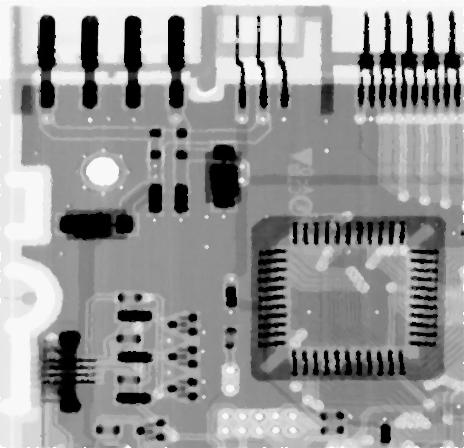
\includegraphics[width=0.5\textwidth]{Assignment_2/output_plots/multipassFilteredImage.png}
    \caption{The result of making 3 passes with a $3 \times 3$ mask with \textit{IPmedian}.}
    \label{fig:IPmedian3pass}
\end{figure}

$^*$Note that some of the images are hard to make out in PDF format, so please run \textit{IPmedian\_test.m} to get the high resolution images.

\newpage
\bibliographystyle{plain}
\typeout{}
\bibliography{Assignment_2}

\appendix
\section{Code}
\subsection{Exercise 1}
\lstinputlisting[caption={exercise\_1.m: Code for exercise 1.}, label={code:exercise1}]{Assignment_2/exercise_1.m}
\subsection{Exercise 2}
\subsubsection{Exercise 2 (a)}
\lstinputlisting[caption={IPfreqrectdists.m: Compute distances to center of $P \times Q$ frequency rectangle.}, label={code:IPfreqrectdists}]{Assignment_2/IPfreqrectdists.m}
\lstinputlisting[caption={IPbhpf.m: Butterworth High-Pass Filter (BHPF).}, label={code:IPbhpf}]{Assignment_2/IPbhpf.m}
\subsubsection{Exercise 2 (b)}
\lstinputlisting[caption={IPftfilter.m: Convolute a filter in the frequency domain.}, label={code:IPftfilter}]{Assignment_2/IPftfilter.m}
\subsection{Exercise 3}
\lstinputlisting[caption={IPmedian.m: Median filter.}, label={code:IPmedian}]{Assignment_2/IPmedian.m}
\end{document}
